\documentclass[
  a4paper,
  % twocolumn,
  % draft
  ]{scrartcl}

% packages

  \usepackage{qbase}

  % extensions

    \bibliography{/Users/quirin/promo/bib/references}

% new commands

  \newcommand{\lsil}[1]{\lstinline[language=Python]{#1}}
  \newcommand{\hw}[1]{\textbf{#1}}
  \newcommand{\mtrc}[1]{\textcolor{blue}{#1}}

\begin{document}

% title

  \title{Social networks of lexical innovation}
  \subtitle{Investigating the diffusion of neologisms on Twitter}
  \author{Quirin Würschinger\\ LMU Munich}
  \maketitle

\listoftodos

\tableofcontents

% text body

\section{Introduction}

  \begin{easylist}[itemize]
    # \hw{Social media} has changed the way we communitate.
      ## It has changed the social fabric of our society (elections, press vs. \enquote{influencers}) and the sociolinguistic dynamics of how we communicate (fake news)
      ## It has also changed the language system and the way the language system changes. Much as \hw{cultural innovations} like XXX \enquote{go viral}, new digital modes of communication also affect the way \hw{linguistic innovations} spread. \todo{technical innovation, example like \ol{blockchain}}
    # This opens up new research questions and new ways to tackle previous questions in sociolinguistics. (sociolinguistics $\rightarrow$ computational sociolinguistics)
      # new data
      # new methods: social network analysis
    # research questions
      # How do new words spread?
      # Which factors influence their spread?
  \end{easylist}

\section{Modeling the conventionalization of lexical innovations}

  \begin{easylist}[itemize]
    # Research question: how do new words spread in the speech community?
    # previous perspectives
      ## \hw{structural}: language system, lexicalization, instutionalization, word-formation processes etc. \cite{Bauer1983,Lipka2005}
      ## \hw{cognitive} \parencite{Schmid2008}
      ## \hw{sociolinguistic}: S-curves \parencite{Labov2007,Milroy1992}
    # current framework: based on the EC-Model \parencite{Schmid2019}
      ## spread across usage contexts
      ## spread across speakers
  \end{easylist}

\section{Investigation the conventionalization of lexical innovations empirically}

  \begin{easylist}[itemize]
    # Previous work has produced some important insights.
    # I focus on the sociolinguistic dimension of lexical innovation in this paper.
    # Previous empirical approaches have been limited to study this because of the lack of information regarding the sociolinguistic dynamics of the spread of new words: how many speakers are affected? how are they interacting?
  \end{easylist}

  Overview of previous approaches

    \begin{easylist}[itemize]
      # traditional corpora \parencite{Elsen2004}
      # web corpora \cite{Renouf2006,Kerremans2012}
        ## linguistic creativity and innovation happen there
        ## big amounts of data
          ### big neologism samples
          ### big corpora (low-frequency nature of neologisms)
        ## more informal sources
      # social media corpora \cite{Grieve2016,Eisenstein2014}
        # hotbed
        # driving force
        # social network information
          ## users
          ## community characteristics
          ## influencers
    \end{easylist}

\section{Going beyond frequency}

  \begin{easylist}[itemize]
    # frequency
    # corpus-as-input \& corpus-as-output, usage intensity \parencite{Stefanowitsch2017}
    # sociolinguistic information
      ## number of users
      ## social network characteristics
      ## influencers
  \end{easylist}

\section{Data}

  \begin{easylist}[itemize]
    # sample
      ## basis: bottom-up selection by NeoCrawler \parencite{Kerremans2018}
      ## extension
        ### quite stable: not topical
        ### reasonably successful: e.g. technical innovations like \ol{blockchain}
        ### sociolinguistically interesting: e.g. political terms such as \ol{covfefe}
    # corpus
      ## longitudinal: retrospective
      ## big data
      ## social network information
  \end{easylist}

\section{Method: social network analysis}

  \begin{easylist}[itemize]
    # basis for networks: interactions between users
      ## mentions
      ## retweets
    # anatomy of a tweet
    # network structure
      ## nodes: users
      ## edges: interactions
  \end{easylist}

\section{Frequency: diffusion trajectories}

  usage intensity serves as a baseline

  \subsection{Sample selection}

    \subsubsection{General sample}

      \begin{easylist}[itemize]
        # clustering: the words can be clustered in these groups \parencite{Kerremans2015}
        # distinguishing between stable and unstable usage: \mtrc{coefficient of variation}
        # distinguishing between degree of success: \mtrc{cumulative usage intensity}
          ## no success
          ## limited
          ## advanced
      # S-curves
        ## we don't expect S-curve trajectories for \hw{topical} neologisms because of variable conceptual salience (c.f. \cite{Nini2017})
        ## for stable neologisms we might expect S-curves \mtrc{model testing for S-curves}
          ### according to sociolinguistic theory we expect certain sociolinguistic dynamics in their spread
          ### in the following sections we will employ social network analysis to empirically test these longstanding hypotheses
      \end{easylist}

    \subsubsection{Case studies}

    \begin{easylist}[itemize]
      # selection criteria
        ## stable
        ## successful
        ## sociolinguistically marked vs. unmarked
      # selection
        ## advanced conventionalization: \ol{shareable}
        ## limited conventionalization:
          ### \ol{alt-right}
          ### \ol{alt-left}
    \end{easylist}

    \begin{figure}[H]
      \centering
      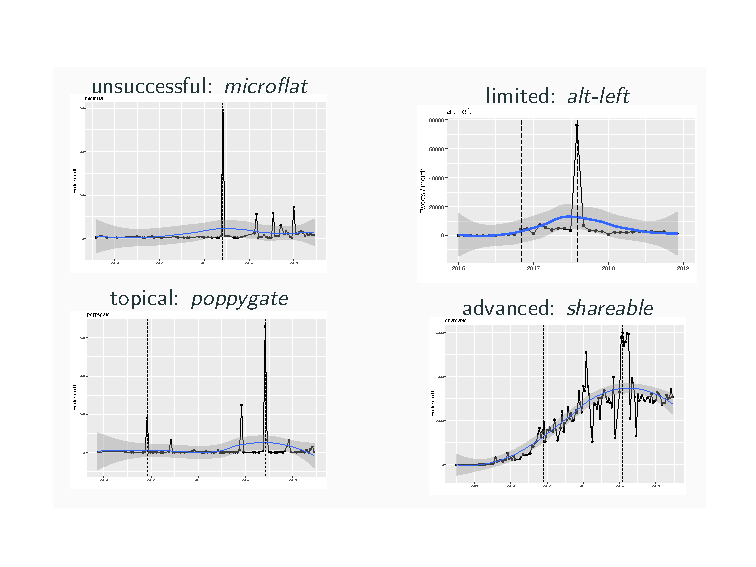
\includegraphics[width=\linewidth, height=.8\textheight, keepaspectratio]{images/ui_cases.pdf}
      \caption{Usage intensity for case studies}
    \end{figure}

    Subsetting

      I subset four stages in the diffusion to zoom in on different phases of the diffusion process \todo{code / plot: mark subsets in plots}

      \begin{easylist}[itemize]
        # first: the first 1,000 attestations
        # mean
        # max
        # last
      \end{easylist}

    I will go beyond frequency and look into the sociolinguistic dynamics more closely

    \begin{easylist}[itemize]
      # sociolinguistic dynamics of diffusion over time
      # sociolinguistic conventionality status of neologism
    \end{easylist}

\section{Diachronic analysis}

  \subsection{Advanced conventionalization: \ol{shareable}}

    \begin{easylist}[itemize]
      # background of \ol{shareable}
        ## linguistic: It's an innocuous formation in that it has a broad meaning and it
          ### form: It's
          ### meaning: broad, diverse scope; significant and stable increase in \enquote{semantic carrying capacity} \parencite{Grieve2016}
        ## diffusion history: first attestations, common uses, etc.
      # template: S-curve
        # shape corresponds quite nicely
    \end{easylist}

    \begin{figure}[H]
      \centering
      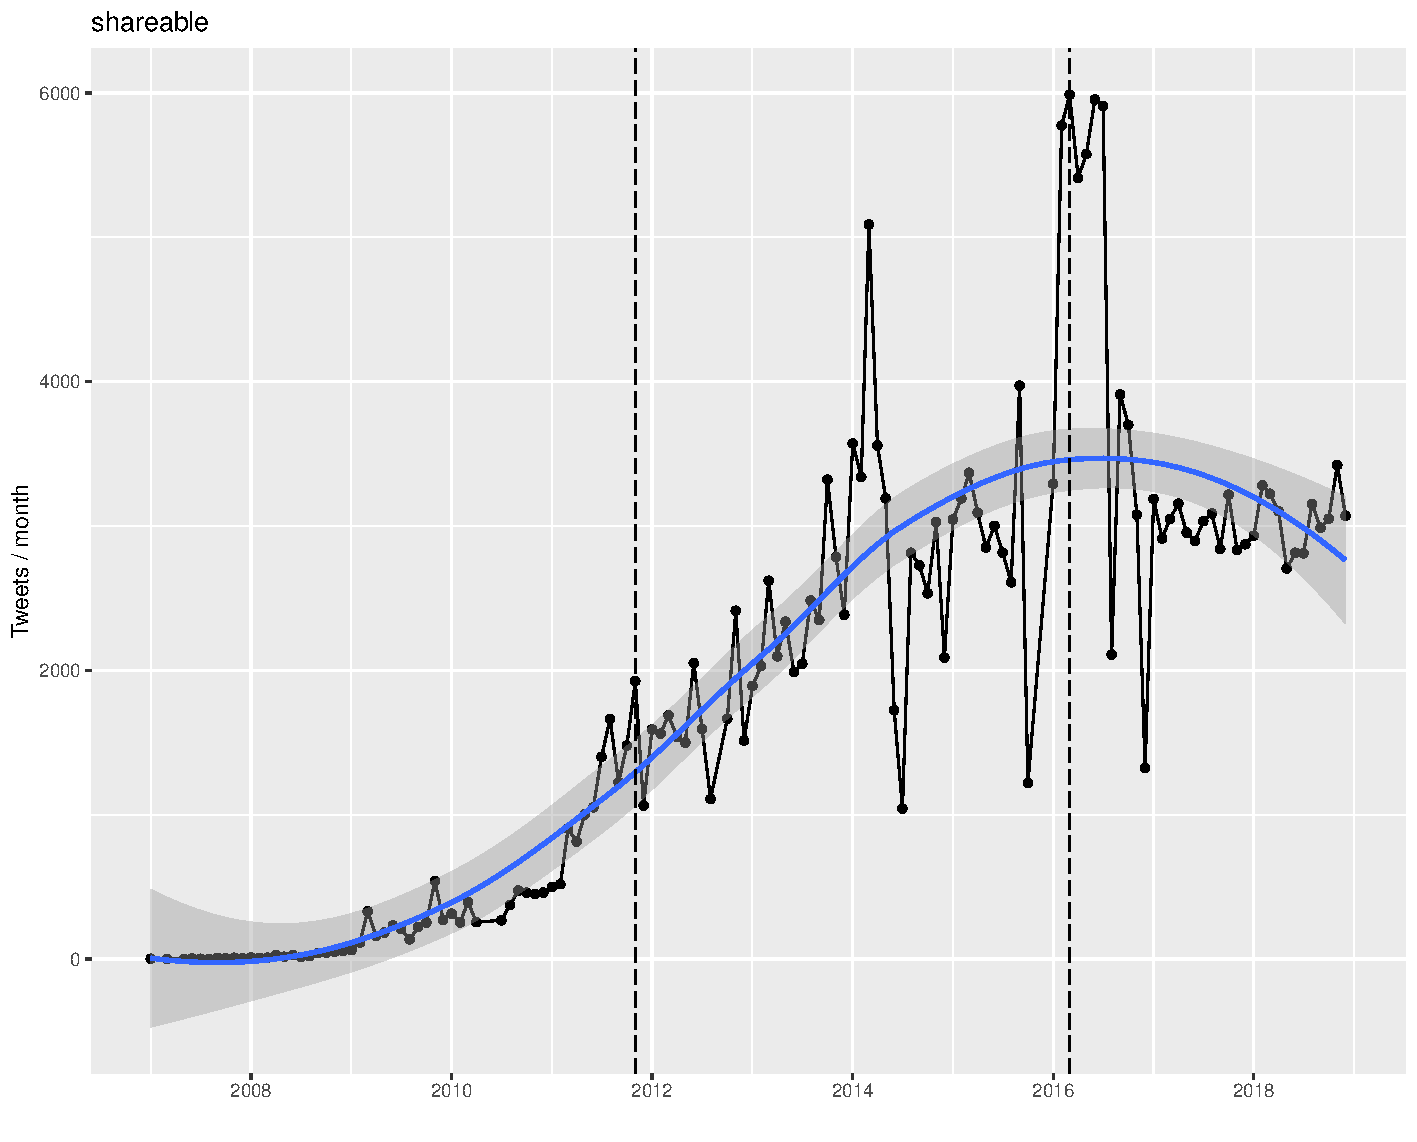
\includegraphics[width=\linewidth, height=.8\textheight, keepaspectratio]{images/ui_shareable.pdf}
      \caption{Usage intensity for \ol{shareable} (n=XXX)}
    \end{figure}

    \begin{figure}[H]
      \centering
      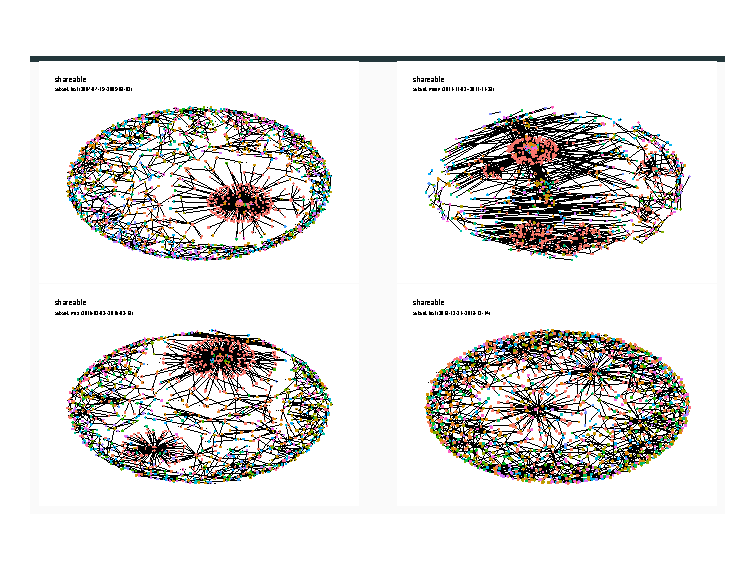
\includegraphics[width=\linewidth, height=.8\textheight, keepaspectratio]{images/net_diac_shareable.pdf}
      \caption{Network over time for \ol{shareable}}
    \end{figure}

  \subsection{No diffusion: \ol{microflat}}

  \subsection{Limited diffusion: \ol{alt-right} and \ol{alt-left}}

    \subsubsection{\ol{alt-right}}

    \subsubsection{\ol{alt-left}}

      \begin{figure}[H]
        \centering
        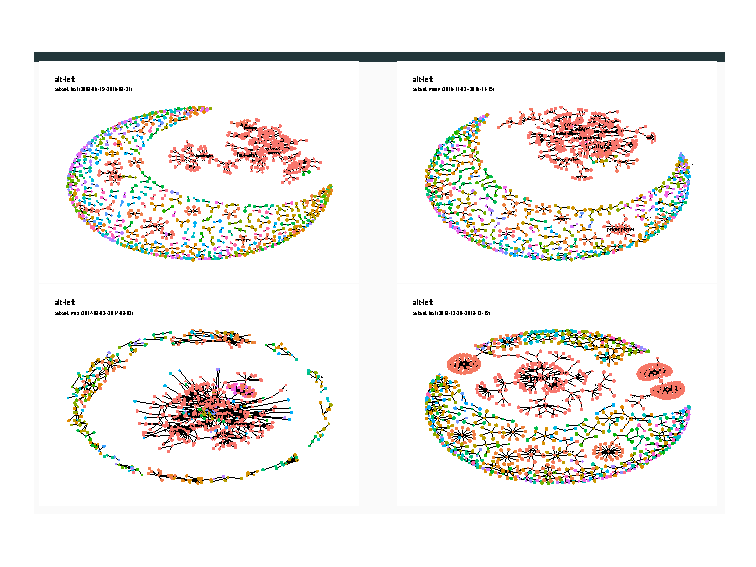
\includegraphics[width=\linewidth, height=.8\textheight, keepaspectratio]{images/net_diac_alt-left.pdf}
        \caption{Network over time for \ol{alt-left}}
      \end{figure}

\section{Synchronic comparison}

  \subsection{Networks}

    \todo{decide: either overall network status or last stage}

    Networks

      last stage

        \begin{figure}[H]
          \centering
          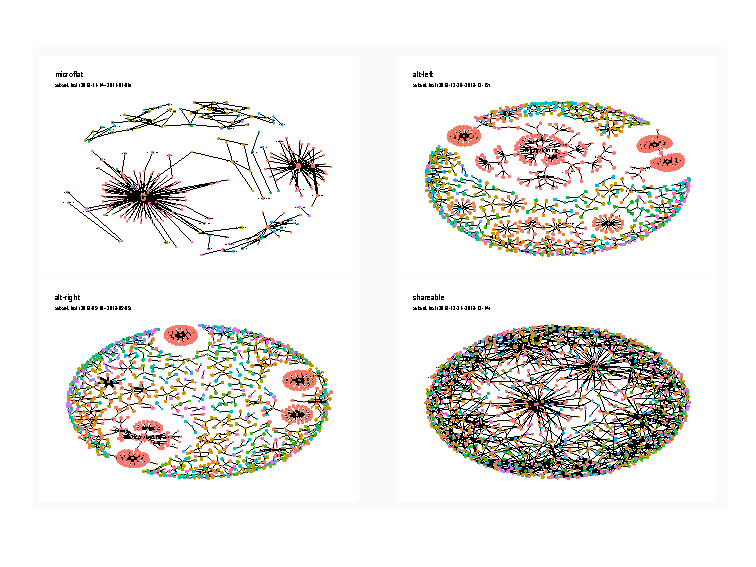
\includegraphics[width=\linewidth, height=.8\textheight, keepaspectratio]{images/net_cases_last.pdf}
          \caption{Network status for case study lemmas}
        \end{figure}

      whole period

        \begin{figure}[H]
          \centering
          \includegraphics[width=\linewidth, height=.8\textheight, keepaspectratio]{images/net_total_alt-left.pdf}
          \caption{Network for interaction across the whole period for \ol{alt-left}}
        \end{figure}

    Metrics

    \begin{figure}[H]
      \centering
      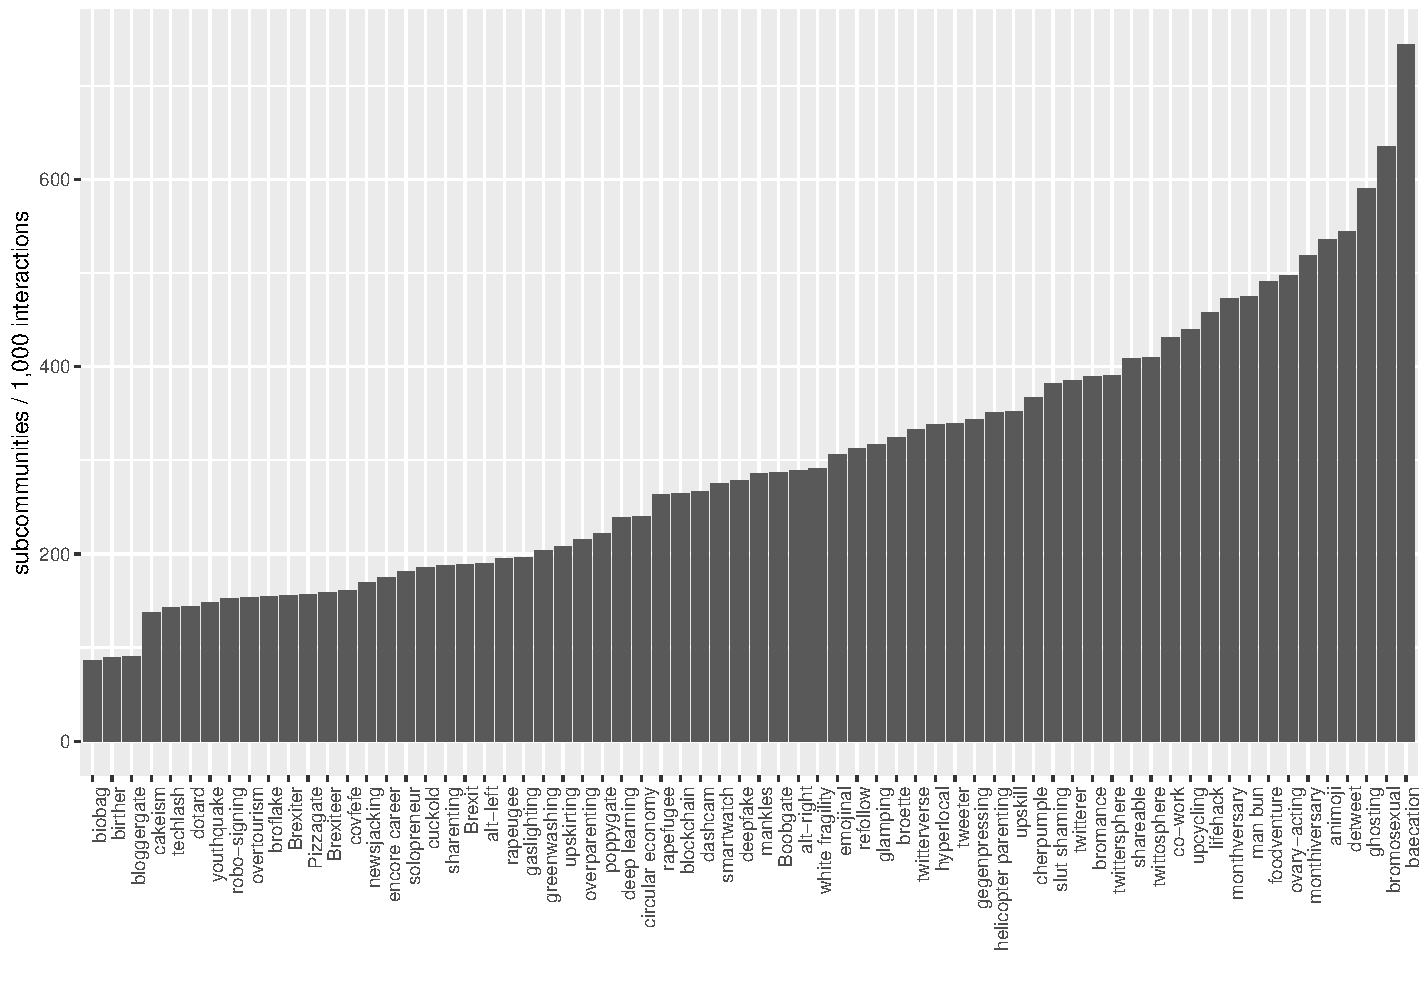
\includegraphics[width=\linewidth, height=.8\textheight, keepaspectratio]{images/communities_last_all.pdf}
      \caption{Network information for all lemmas}
    \end{figure}

  \subsection{Usage intensity}

    \begin{figure}[H]
      \centering
      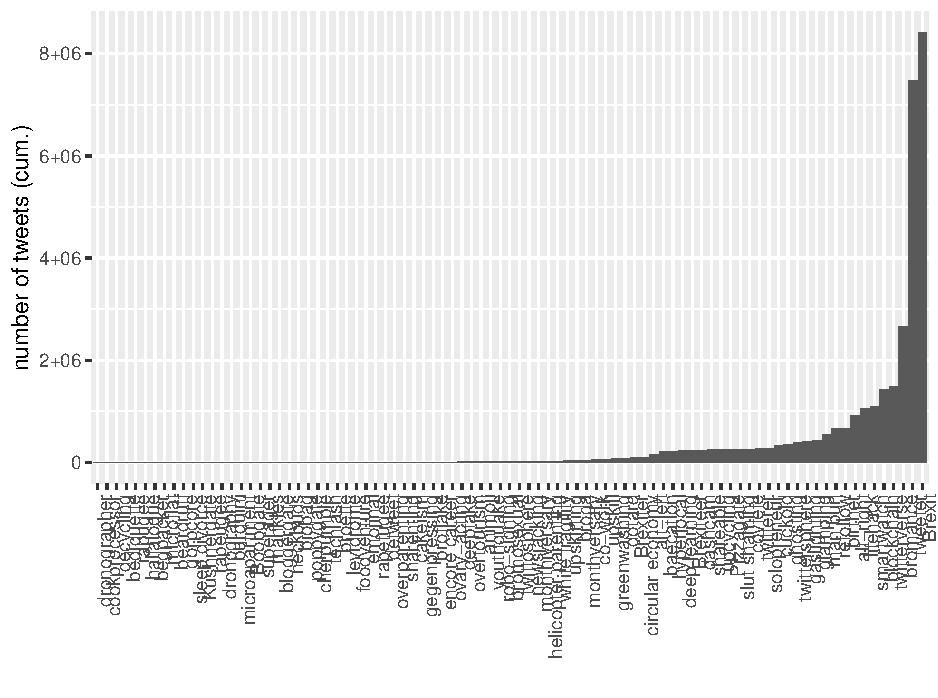
\includegraphics[width=\linewidth, height=.8\textheight, keepaspectratio]{images/comp_ui_all_cum.pdf}
      \caption{Cumulated frequency counts for all lemmas}
    \end{figure}

  \subsection{Networks and usage intensity}

    Grouping and interpretation

      \begin{easylist}[itemize]
        # advanced
        # topical
        # little dispersion
          ## political camps:
            ### propaganda: \ol{alt-right}, \ol{alt-left}, \ol{covfefe}, \ol{birther}
            ### Brexit terms: \ol{Brexiteer}, \ol{Brexiter}, \ol{Brexit}
          ## technical
      \end{easylist}

      \begin{figure}[H]
        \centering
        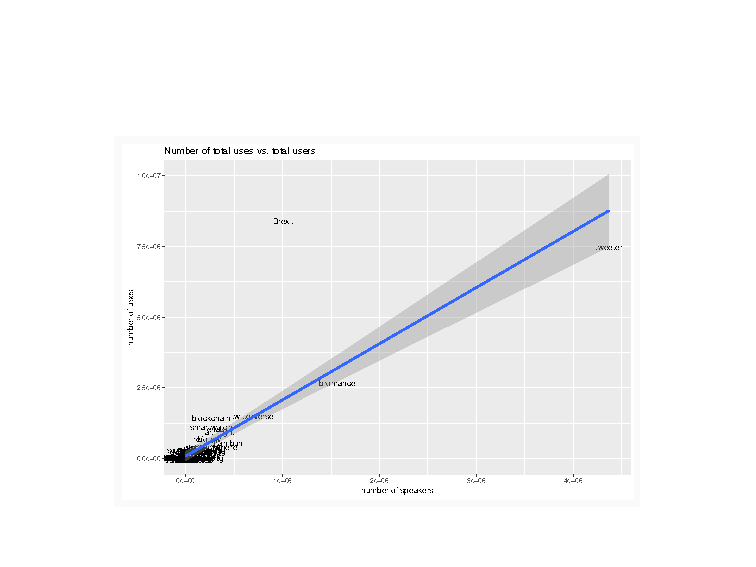
\includegraphics[width=\linewidth, height=.8\textheight, keepaspectratio]{images/users-vs-usage.pdf}
        \caption{Users vs. usage}
      \end{figure}

% bibliography

  \printbibliography

\end{document}
